\section{GPU Architectures and CUDA}\label{sec:GPUsCUDA}
The most widely GPUs used for High Performance Computing are those produced by NVIDIA. The architecture of these GPUs is based on a set of Streaming Multiprocessors (SMs), each containing Streaming Processors (SPs), a set of Special Function Units (SFUs) and a number of load/store (LD/ST) units. The multiprocessors execute threads asynchronously, in parallel. The SM schedules threads in groups of 32 parallel threads called warps, which can use LD/ST units concurrently, allowing simultaneous reads and writes to memory. Above the main parts of a GPU is explained:

\begin{itemize}
    \item Graphic Processing Clusters (GPC): TPC is a chip which grouped the streaming multiprocessor in a GPU. Single GPC contains a raster engine. It is a way to encapsulate all key graphics processing units. Before to Fermi, SMs and Texture Units were grouped together in hardware blocks called Texture Processing Clusters (TPCs). But after Fermi, SMs have dedicated Texture Units. 
    
    \item Streaming Multiprocessors (SM): A SM is designed to execute thousands of threads concurrently, up to 2048 threads on recent architectures. To manage such a large amount of threads, the instructions are pipelined through simultaneous hardware multithreading. These hardware units are SP, SFU, LD/ST, among others. The smallest executable unit of parallelism on a NVIDIA device is 32 threads or a warp. Normally different architectures have a different number of SMs and the number of hardware units inside it. 
    
    \item Hardware units: Streaming multiprocessor are commonly organized by FP32 and FP64 cores, SFU and LD/ST units. FP32 and FP64 cores are shaders processors which are designed to do streaming floating point calculations. SFUs are special function unit for "fast approximate transcendental operations". They execute transcendental instructions such as \textit{sin}, \textit{cosine} and \textit{square root}, with each SFU executing one instruction per clock. Load/Store units are used to read and write in the global memory. One instruction can read/write up to 128 bytes, as a consequence, if each thread in a warp reads 4 bytes and they are coalesced, then whole warp would require a single load/store instruction. If accesses are uncoalesced, then more transaction should be issued.
    
\end{itemize}

Until now, the GPU architectures manufactured by NVIDIA are Tesla, Fermi, Kepler, Maxwell, Pascal and recently Volta. Generally, the hierarchical memory of a NVIDIA GPU contains global and shared portions. Global memory is large, an off-chip, has a high latency and can be accessed by all threads in the GPU. Shared memory is small, on-chip on each SM, has a low-latency and can be accessed only by threads in the same SM. Each SM has its own shared L1 cache and an off-chip coherent global L2 cache. 

All NVIDIA architectures vary in a large number of features, such as the number of cores, registers, SFUs, load/store (LD/ST) units, cache memory sizes, processor clock frequency, memory bandwidth, unified virtual memory, and dynamic parallelism. One main challenge in the designing of new generations of massively parallel architectures is the ratio of improvement between energy consumption and performance~\citep{Mittal:2014}. 
Those differences are summarized in the Compute Capability (C.C.) of NVIDIA GPUs, shown in Table~\ref{tab:CC}. Many of these differences will be exposed in Subsection \ref{ssec:GPUroadmap}, where we mention some technical specifications of each NVIDIA GPU architecture.  

\subsection{NVIDIA GPU Roadmap}\label{ssec:GPUroadmap}

\paragraph{Tesla Architecture:}
This architecture was one of the first GPU to support C or CUDA, allowing programmers to use these devices without having to learn a new programming language. 
Currently, Tesla is also the name of the GPUs designed for High Performance Computing. 

The model GeForce 8800 was one of the first model designed with this architecture, see Figure~\ref{fig:GTX:8800}. This GPU has 112 SP, these SPs were grouped in seven independent chips called Texture/Processor Clusters (TPCs)~\citep{2008:TeslaGPU}. Each TPC has 2 SM and each SM consists of eight streaming processors, 16KB of on-chip shared memory, two SFUs, a constant cache, a multithreaded instruction fetch and issue unit and a read-only constant cache. Second versions of Tesla architectures implemented fused multiply-add (FMA) for double precision.

\begin{figure}[htpb]
\centering
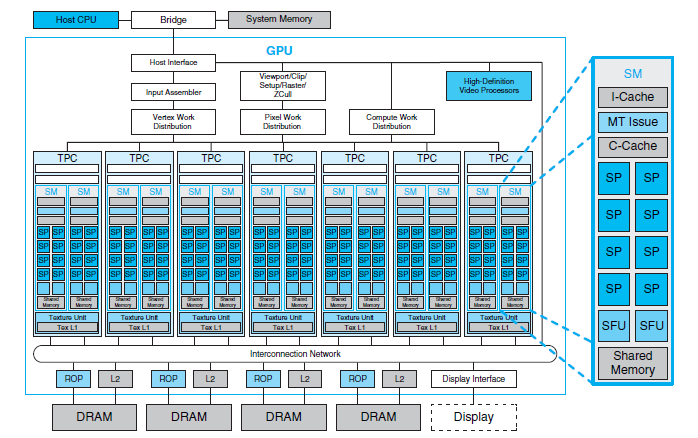
\includegraphics[scale=.85]{images/GeForce-8800-GTX-2-1.png}
\caption{GPU GeForce GTX 8800, the first to support CUDA platform, extracted  from NVIDIA Documentation}
\label{fig:GTX:8800}
\end{figure}

\paragraph{Fermi Architecture:} Fermi architectures implemented the IEEE 754-2008 floating-point standard \citep{FMA-IEEE} for both single and double precision arithmetic which performs multiplication and addition with a single rounding step. In this architecture is possible to have a second-level cache L2 shared by all SMs and each SM has a memory cache L1.

A NVIDIA's Fermi GF-100 has 4 GPC, each GPC has 4 SMs for a total of 16 Streaming Multiprocessors. Each SM is composed of 32 cores, resulting in a total of 512 cores. It also has 4 SFUs, 2 warp schedulers, and 16 LD/ST units. Now it has configurable cache L1 or shared memory of 64KB, these configurations can be of 48 KB of shared memory and 16 KB of L1 cache or 16 KB of shared memory and 48KB of L1 cache. 

Among the most important characteristics of programmability of this architecture were to allow concurrent kernel execution, out of order thread block executions and dual overlapped memory transfer engines.

\paragraph{Kepler Architecture:}
In this architecture, the abbreviation for SM changed to SMX. Each SMX has 4 warp schedulers and eight instruction dispatch units, allowing four warps to be issued and executed concurrently. Unlike Fermi, Kepler architectures allow double precision instructions to be paired with other instructions. The shared memory continues sharing the same chip than L1 cache and the same size, 64KB, but now this architecture allowed the configuration of the shared memory and cache memory L1 in different 3 sizes. The 3 different configurations in KB for shared memory and L1 cache are 48/16 32/32 or 16/48. Kepler also introduced a 48KB of cache for read‐only data for SM. 

The GeForce GTX 680 GPU consists of four GPCs, each one of 4 SM for a total of 16 Streaming Multiprocessors. Each SM is composed of 192 cores, resulting in a total of 1536 cores. It has also 32 SFU, 4 warp scheduler and 32 LD/ST units. 

Among the most important characteristics of programmability of this architecture were the addition of dynamic parallelism and hyper-Q. Dynamic Parallelism allowed the GPU to create new work for itself, synchronize on results, and control the scheduling without involving the CPU. Hyper-Q enables different host threads to trigger execution of kernels simultaneously, in the Kepler architecture 32 concurrent connections are possible with the CPU. 


\paragraph{Maxwell Architecture:} 
The L1 cache is shared now with the texture cache with a size of 24 Kb. Unlike in Kepler and Fermi, the Maxwell architecture has a dedicated shared memory and does not share level with the level 1 cache. The shared memory now is a dedicated chip of 96 KB. Scheduling algorithms have been rewritten to avoid stalls\footnote{stalls is a delay before the processor can continue to execute a statement}, thus reducing the amount of energy spent per instruction. 

GPU Maxwell GM204 consists of four GPCs, each one of 4 SM for a total of 16 Streaming Processors. Each SM is composed of 128  cores, resulting in a total of 2048 CUDA cores. This time, the SMs are partitioned into 4 blocks, each with its instruction buffer, its scheduler. Each block also has 8 LD/ST units, 8 SFU. 
The main features introduced by the Maxwell architecture are related to power consumption and Unified Virtual Addressing (UVA). UVA allows direct access between the host and the devices, without requiring a buffer in the host to perform data transfer.

\paragraph{Pascal Architecture:}
Pascal architecture brings big changes in NVIDIA GPUs, it introduces the new technology of stacked DRAM memory and it brings a new technology of interconnection between GPUs named NVlink. Another important characteristic of this architecture is the addition of preemption, now GPU applications are available to do preemption during their executions. 

Pascal continues which the groups of multiprocessors in GPC and the dedicated chip for shared memory per Streaming Multiprocessors. Cache L1 continues sharing the same chip than Texture cache, but the size increased to 48KB.

\paragraph{Volta Architecture:} This architecture has came optimized for Deep Learning applications. Save energy has been an important parameter in the design of this architecture, in comparison with Pascal GPUs the new Volta SM is 50\% more energy efficient than the previous Pascal architecture. This architecture introduces a new characteristic, this characteristic is named \textbf{Tensor Cores}. Shared memory back to be combined with a L1 cache memory. This chip-on memory increased its size and it is now of 124 MB and shared memory is configurable up to 96 KB.

A Volta GV-100 has 6 GPC, each GPC inside has 14 SMs and each SM has 64 SP for a total of 5376 cores. The GV100 SM is partitioned into four processing blocks, each with 16 FP32 units, 8 FP64 units, two tensor cores for deep learning matrix arithmetic, one warp scheduler and one dispatch unit. 

One of the main characteristics in the programmability is the concept of Cooperative Groups, the is a new programming model for organizing groups of communicating threads, it allows developers to express the granularity at which threads are communicating. Table~\ref{tab:CC} shows a better summary of the main Tesla GPU architectures manufactured by NVIDIA.


\begin{table}[htpb]
    \centering
    \begin{tabular}{|r|c|c|c|c|c|}
    \hline\hline
        {\bf Features/Teslas}&{\bf Fermi}&{\bf Kepler}&{\bf Maxwell}&{\bf Pascal}&{\bf Volta}\\\hline
        % Features&Fermi GF100&Kepler GK110&Maxwell GM200&Pascal GP100\\\hline
         Compute Capability&2.0&3.5&5.3&6.0&7.0\\\hline
        %  SMs per GPCs&1&1&4&10&14\\\hline
         SMs &13&15&24&56&84\\\hline
         SPs per SM &32&192&128&64&64\\\hline
         FP32 Units&512&2880&3072&3840&5376\\\hline
         FP64 Units &-&512&960&1792&2560\\\hline
        %  FP64 Units &-&512&960&1792&2560\\\hline
        %  Memory Interface&384-bit GDDR5&384-bit GDDR5&384-bit GDDR5&4096-bit HBM2&4096-bit HBM2\\\hline
         Max Warps per SM&48&64&64&64&64\\\hline
         Max Thread per SM&1536&2048&2048&2048&2048\\\hline
         Shared memory size (KB)&48&48&96&64&up to 96\\\hline
         Manufacturing process (nm)&40&28&28&16FinFET&12 FinFET\\\hline
         Hyper-Q&No&Yes&Yes&Yes&Yes\\\hline
         Dynamic Parallelism&No&Yes&Yes&Yes&Yes\\\hline
         Unified Memory&No&No&No&Yes&Yes\\\hline
         Preemption&No&No&No&Yes&Yes\\\hline\hline
          
    \end{tabular}
    \caption{Description of the Compute Capability of the last GPU NVIDIA architectures}
    \label{tab:CC}
\end{table}

On the left side of Figure~\ref{fig:hierarchyThread} is shown the memory hierarchy of a thread that runs on a GPU with Fermi architecture. In this architecture, the L1 cache is in the same chip than shared memory. On the middle is shown the memory hierarchy of a thread that runs on a GPU with Kepler or Volta architecture, in this architecture a cache read-only is added and the L1 cache is in the same chip than Shared memory. In the right side is shown a memory hierarchy of a thread which runs on a GPU with Maxwell or Pascal architecture, in these architectures the shared memory is dedicated and the L1 cache is in the same chip than a texture cache. Figures were modified from the NVIDIA documentation.

\begin{figure}[htpb]
\centering
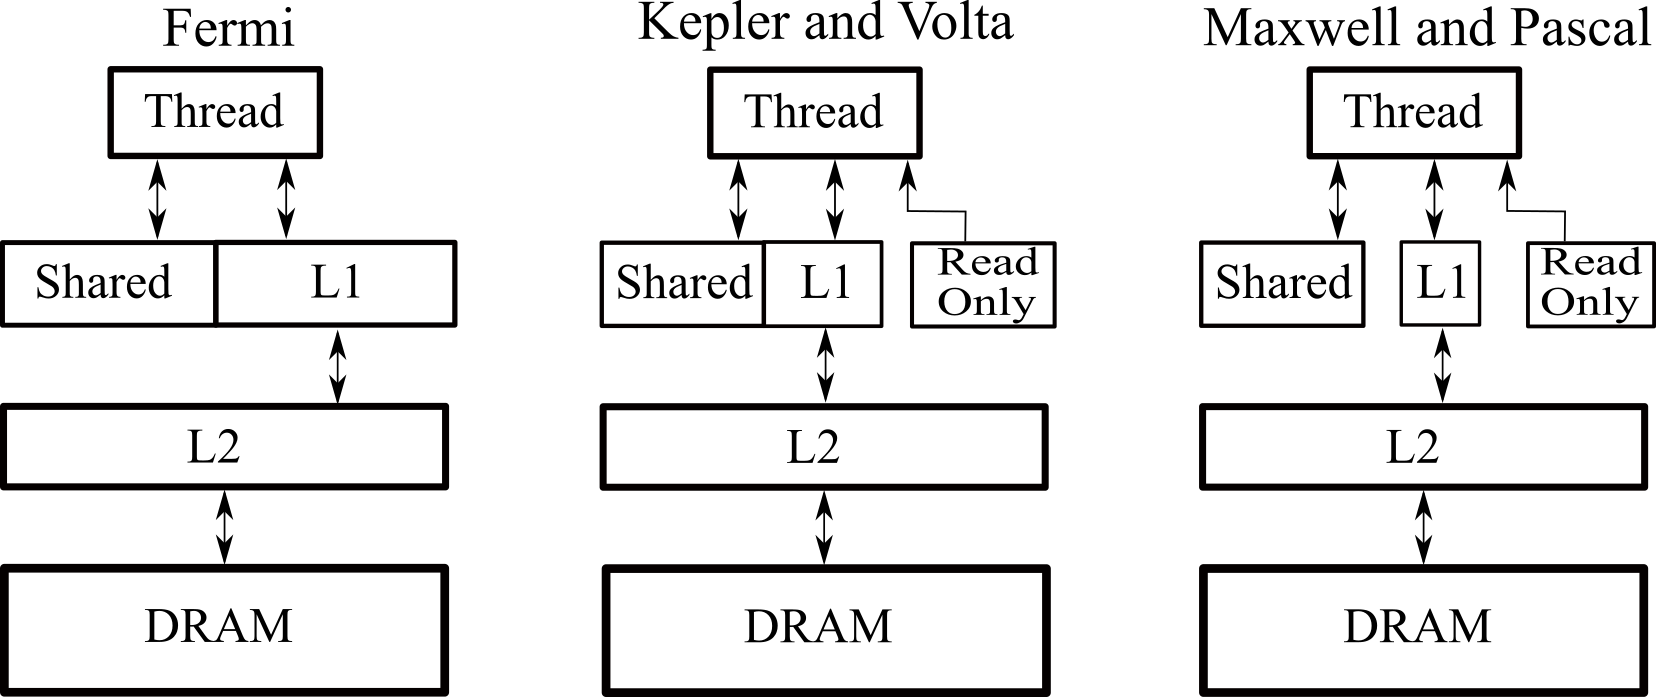
\includegraphics[scale=.25]{./images/hierarchyThread.png}
\caption{Left: Memory hierarchy accessed from a thread in a GPU with Fermi architecture. Right: Memory hierarchy accessed from a thread in a GPU with Kepler architecture}
\label{fig:hierarchyThread}
\end{figure}

\subsection{\textit{Compute Unified Device Architecture} (CUDA)}\label{ssec:CUDA}
The parallelism reached by the GPUs of NVIDIA is of the type Single Instruction Multiple Data (SIMD), but commonly NVIDIA denominates this type of parallelism \emph{Single Instruction Multiple Threads} (SIMT), where thousands or millions of threads are executed concurrently into the GPU. In the type of parallelism used by the SIMT, an application launches a function with many threads which will execute the same instructions, and threads are programmed dynamically in a SIMD-like parallelism to access data.  By itself, SIMD only describes how the instructions are executed. 

The SIMT programming model has an approach that is different from the traditional \textit{multicore} processor model. In particular, the Open Computing Language (OpenCL) is a low-level API for writing programs that can execute across heterogeneous computing systems (i.e., consisting of GPUs and CPUs) and even other kinds of processing units. CUDA and others tools provide ways to parallel computing using data-based or task-based parallelism on different architectures. CUDA works in a single-instruction multiple-data parallelism, where data is accessed by the index of each thread in a CUDA function.

The CUDA platform enables the use of NVIDIA GPUs for scientific and general purpose computation. A single \textit{master} thread runs in the CPU, launching and managing computations on the GPU. GPUs have their own memory and data must be transferred through a PCI Express bus. Data for the computations have to be transferred from the host memory to the device memory. Actually, the execution flow of a GPU application can be divided into three key stages. First, data is transferred to the memory of the GPU; in a second stage, the main program executed on the CPU (called host) is responsible for starting threads in the GPU (called device), launching a function (called kernel). Finally, results are sent back to the host. Figure~\ref{fig:cuda:model} shows a classical execution workflow of a CUDA application.

\begin {figure}[htpb]
  \centering
  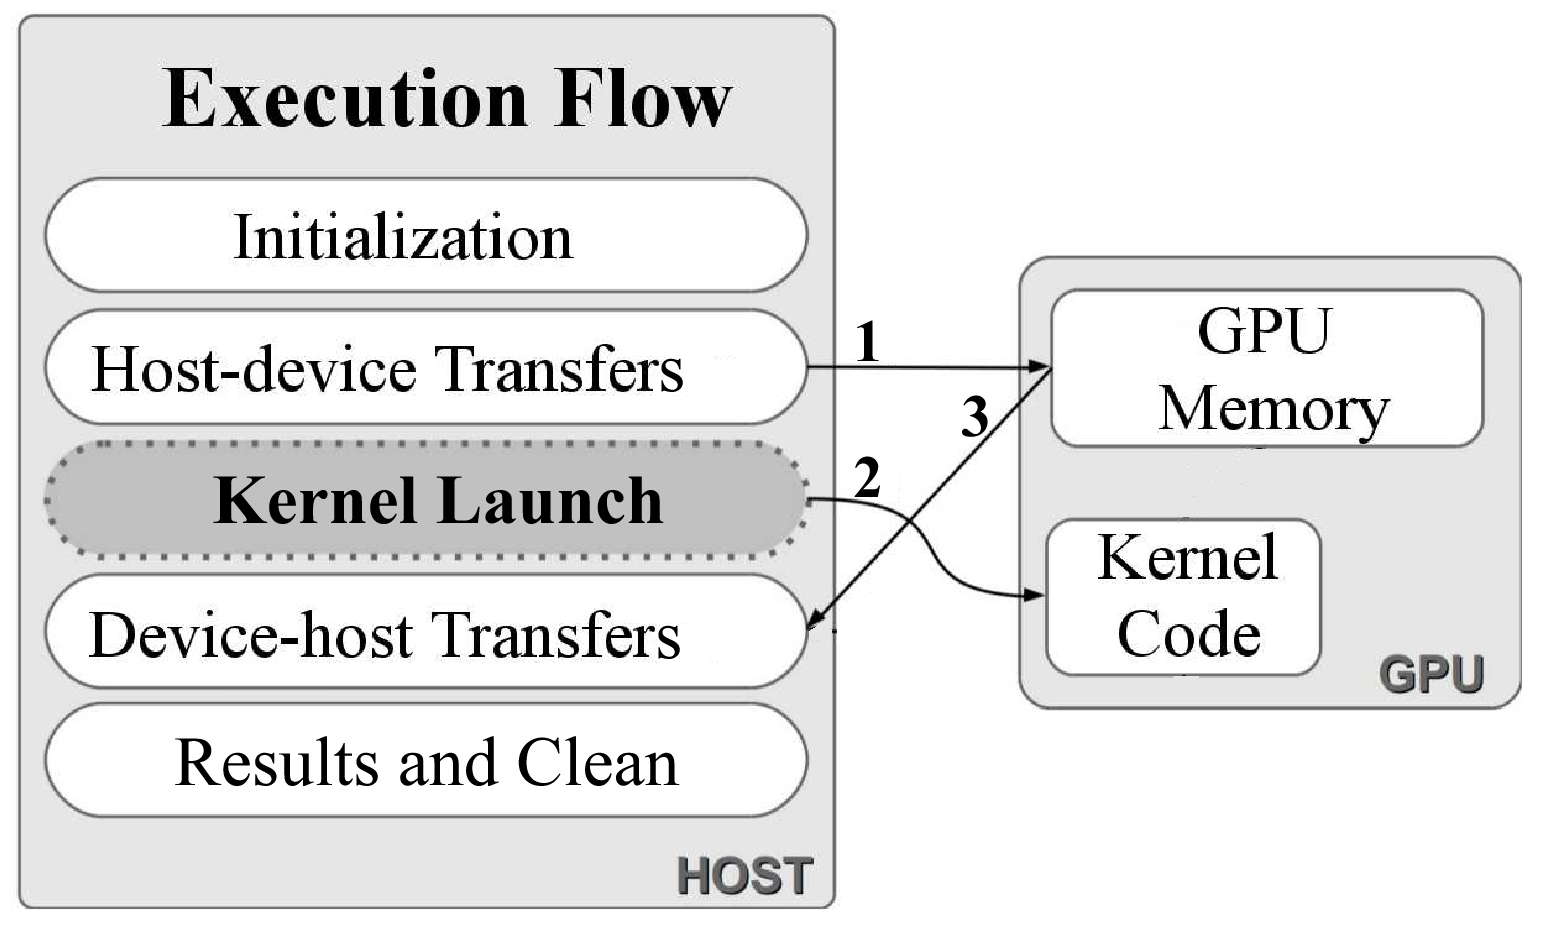
\includegraphics[width =.45\textwidth] {images/modelo-classico-execucao.png}
  \caption{Classical Execution of a GPU application}
  \label{fig:cuda:model}
\end {figure}

The CUDA language extends C and provides a multi-step compiler, called \texttt{NVCC}, that translates CUDA code to Parallel Thread Execution code or \emph{PTX}. \texttt{NVCC} uses the host's C++ compiler in several compilation steps, and also to generate code to be executed in the host. The final binary generated by \texttt{NVCC} contains code for the GPU and the host. When \texttt{PTX} code is loaded by an application at run-time, it is compiled to binary code by the host's device driver. This binary code can be executed in the device's processing cores and is architecture-specific. The targeted architecture can be specified using \texttt{NVCC} parameters~\citep{CUDAGuide}. 

When a kernel is launched, $t$ parallel threads are executed into the CUDA cores of a GPU. All threads execute a copy of the same code defined in the body declaration of the kernel function. The number of threads in a kernel is defined in two tri-dimensional parameters. The number of threads in a block and the number of blocks in a grid, the special words in CUDA to define those parameters are \texttt{blockDim} and \texttt{gridDim}, respectively. Each kernel create a grid of threads into the GPU, each grid is organized by blocks and these blocks are divided by threads, see Figure~\ref{fig:dimGridBlock}. It is normal to associate the dimension of the block to the dimension of the problem to solve.

\begin{figure}[htpb]
    \centering
    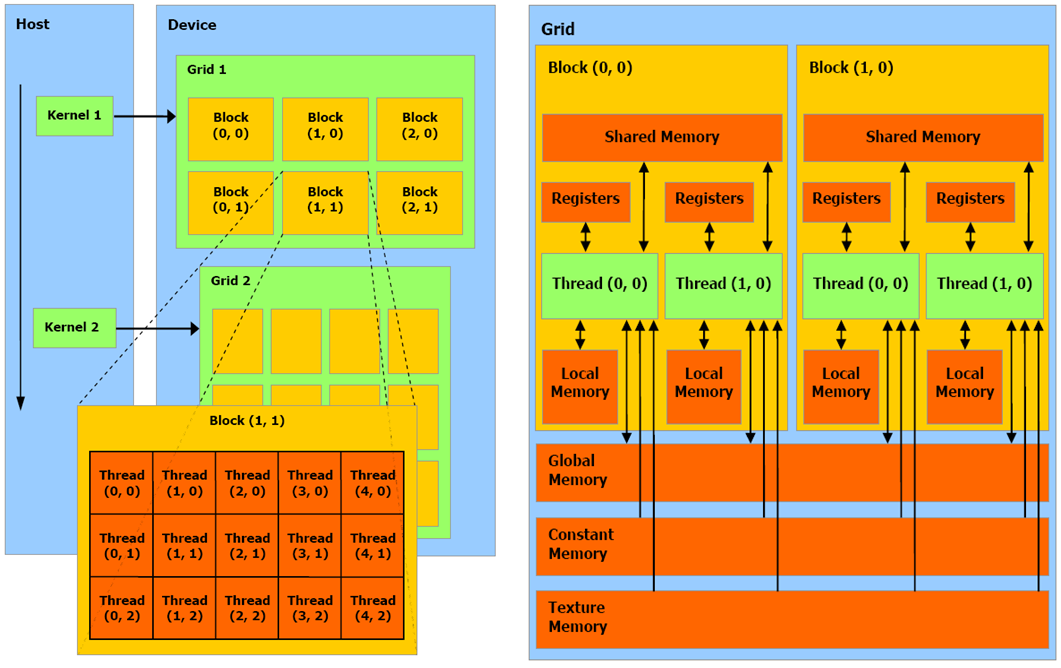
\includegraphics[scale=.85]{images/Kernel-grid-organization.png}
\caption{Thread hierarchy and memory visibility of a kernel, copied from NVIDIA Documentation}
\label{fig:dimGridBlock}
\end{figure}

Threads in a grid have access to different memory types. Threads in the same block can access with a high bandwidth to registers, shared memory and local memory, i.e. on-chip memory in the SM. All threads in the grid have access to load and write in the global, but only to load from the constant and texture memory, see Figure~\ref{fig:dimGridBlock}. Threads can be synchronized on two different levels, global memory, and shared memory. Thread into the same block can be synchronized across the shared memory with a high bandwidth. All threads in a kernel are synchronized across the global memory with a bandwidth lesser than shared memory, resulting in an expensive instruction for GPU applications.

The maximum number of threads in a block or blocks in a grid is specific for each compute capability, these values are shown in Table~\ref{tab:CC}. something to notice In this table is the number of SPs per SM which increase in the Kepler architecture and after decreases in the next architectures; and the number maximum of warp per SM increase in Kepler and it keeps  the same (64) in posterior architectures. This ensures a better occupancy of the SM.

If threads of the same warp execute different instructions, i.e. warps executing a conditional statement, the CUDA compiler must generate code to branch the execution correctly, making the program lose performance due to this \emph{warp divergence}. Code divergence greatly degrades the performance of an application running on such architectures. 

The bandwidth of the global memory can be largely improved by combining the LD/ST requests from different threads of a single warp, in a process called coalescing~\citep{confwdagHaTA08}. The coalescing occurs when the threads access contiguous global memory addresses, which permits usage of the multiple LD/ST units available per SM.% All the levels of the memory hierarchy are benefited by this communication optimization.

Multiple computations launched by the master thread, or \textit{kernels}, can run asynchronously and concurrently in a current GPU. In CUDA, all kernel executions are asynchronous, threads of the same block can be synchronized with the function \texttt{{\_\_}syncthreads()} and the function \texttt{cudaThreadSynchonize()} can synchronize all the threads of a kernel or grid. 

Finally, all threads of a grid are mapped, and receive identifiers corresponding to the declared dimensions. These identifiers
are available and accessible in CUDA code through variables such as \texttt{threadIdx} and \texttt{blockIdx}. This allows the execution, identification and control of threads in a GPU. The identifiers \texttt{threadIdx.x}, \texttt{threadIdx.y} and \texttt{threadIdx.z} are associated with the threads within a block and \texttt{blockIdx.x}, \texttt{blockIdx.y} and \texttt{blockIdx.z} are associated with the index of a block within a grid.

In the next section, we describe each one of the kernels used as benchmarks in this research and discuss main characteristics of communication and computation of each one. 
